%-------------------------------------------------------------------------------
% yum_midi_learn
%-------------------------------------------------------------------------------
%
% \file        yum_midi_learn.tex
% \library     Documents
% \author      Chris Ahlstrom
% \date        2016-12-22
% \update      2018-05-16
% \version     $Revision$
% \license     $XPC_GPL_LICENSE$
%
%     Provides the midi_learn section of yoshimi-user-manual.tex.
%
%-------------------------------------------------------------------------------

\section{MIDI Learn}
\label{sec:midi_learn}

   \index{MIDI Learn}
   \index{midi!learn}
   In this section, we show how to use the new (with 1.5.0)
   \textbf{MIDI Learn} feature of \textsl{Yoshimi}.
   MIDI Learn is a method to remotely control many parameters in an audio/MIDI
   application via a MIDI controller.  Each parameter that is "learned" can be
   controlled, and the setting changes recorded.

\subsection{MIDI Learn / Basics}
\label{subsec:midi_learn_basics}

%   In \textsl{Yoshimi}'s direct-access system, MIDI Learn is available, to
%   the extent that it can handle controls that have a range of 0 to 127.

   One can have multiple controls on the same CC.  But, although they all work,
   only the last one updates the user interface.  They are channel specific. So
   if one is rich enough to have two MIDI keyboards, one can set them up to do
   quite different jobs.
   Some of the controls, like volume and pan, are immediate, but most are "next
   note".

   In order to unset a learned value, simply delete the line.
%  One cannot get them to block others on the same
%  CC/channel pair; that will come later.

   Some external controllers use the pitch wheel control per-channel for up to 16
   high-resolution faders.
   Some synthesizers send a number of high resolution controllers as NRPNs.
   \textsl{Yoshimi} MIDI Learn can handle these.
   The controls that can actually benefit from better resolution are
   most of the volume and detune ones.
   They are learned in exactly the same way as ordinary CCs, but instead of
   presenting a line that includes an editable CC field, they show a non-editable
   hexadecimal number with a space between the bytes and followed by an "h",
   such as \texttt{0a 2c h}.
   Also, these lines default to having \textbf{Block} set.
   See that item's discussion below.

   Now \textsl{Yoshimi} can respond to aftertouch.
   One might wonder why one would want to MIDI-learn modulation when there is
   already a dedicated CC for it; and the same for "brightness". The answer is
   that there is currently no way to link these to aftertouch, and this is
   especially relevant for people using wind controllers.
   MIDI Learn sees aftertouch as CC 129 (via a sneaky conversion).
   This has another nice result.
   If one does not have an aftertouch device currently
   in hand, use any other controller; then, in the editing window, just change
   the controller number to 129. Save the learned set, and next time one
   \textsl{does} have such a device, just load the file and off you go!  MIDI
   Learn can emulate the MOD wheel, as it is an accessible control in the
   little panel brought up when one right-clicks the \textbf{Controllers}
   button in the bottom panel of the \textsl{Yoshimi} main window: One can use
   it for any volume or pan, and can have a lot of fun with things like the
   \textbf{Phaser} effect as these are all "instant".  The \textbf{Mod} wheel
   is seen as CC 130.

   Finally, there is a hidden control that can be learned, \textbf{Breath} (CC 2).
   This will show in the learned list, but there is no GUI knob to represent it.

\begin{figure}[H]
   \centering
%  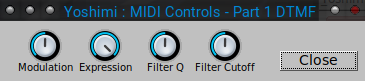
\includegraphics[scale=1.0]{1.5.3/midi-controls-panel.png}
   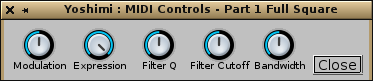
\includegraphics[scale=1.0]{1.5.4/MIDIcontrols.png}
   \caption{MIDI Controls Panel}
   \label{fig:midi_controls_panel}
\end{figure}

   The emulated \index{MIDI controls} MIDI controls are:
   \index{Modulation} \textbf{Modulation},
   \index{Expression} \textbf{Expression},
   \index{Filter Q} \textbf{Filter Q},
   \index{Filter Cutoff} \textbf{Filter Cutoff}, and
   \index{Master Bandwidth} \textbf{Master Bandwidth}.

\subsection{MIDI Learn / User Interface}
\label{subsec:midi_learn_user_interface}

   To activate MIDI Learn, \texttt{Ctrl-right-click}
   on any user interface control.
   A pop-up window will detail the control selected, or indicate that the
   control is not learnable.
   A message will also appear in the console window or command-line interface
   (if active).

\begin{figure}[H]
   \centering
   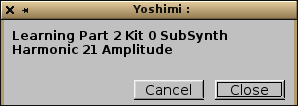
\includegraphics[scale=0.75]{1.5.0/Learning-30amp.png}
   \caption{MIDI Learn Prompt Example 1}
   \label{fig:midi_learn_ex_1}
\end{figure}

   Here is another example:

\begin{figure}[H]
   \centering
   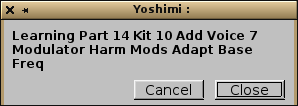
\includegraphics[scale=0.75]{1.5.0/Learning-Mods.png}
   \caption{MIDI Learn Prompt Example 2}
   \label{fig:midi_learn_ex_2}
\end{figure}

   If a \texttt{Yoshimi} control is not MIDI-learnable, a message pop-up
   will indicate that it is not
   learnable:

\begin{figure}[H]
   \centering
   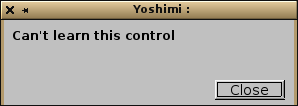
\includegraphics[scale=0.75]{1.5.0/Learning-No.png}
   \caption{MIDI Learn Prompt Unsupported Example}
   \label{fig:midi_learn_unsupported}
\end{figure}

   \index{midi!learn, slider quirk}
   Note that the majority of controls, including the sliders, are MIDI
   learnable.  However, also note that, for sliders to be learned, one must
   click on the \textsl{track} of the slider, not the \textsl{thumb} of the
   slider.

   If the \textsl{Yoshimi / Midi Learn} button is pressed, and there are no
   MIDI-learn entries available yet, then the following empty dialog appears:

\begin{figure}[H]
   \centering
   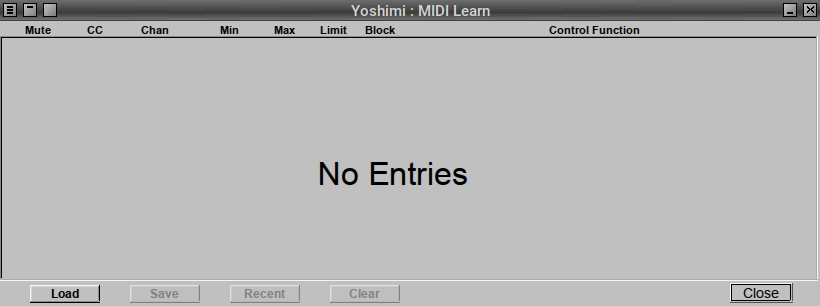
\includegraphics[scale=0.50]{1.5.0/MidiLearn-empty.png}
   \caption{Empty Midi Learn Dialog}
   \label{fig:empty_midi_learn_dialog}
\end{figure}

   A message will also appear in the console window/CLI.

   After turning on learn, the first physical controller moved, or CC message
   sent, will be locked in, and one will see the user-interface knob or slider
   move in synchrony with the physical control. The pop-up window will
   disappear, and the console message \texttt{Learned} appears, with a line
   underneath with exactly what control was caught.

   There is also an activity "LED" between \textbf{Chan} and
   \textbf{Min} indicators that flickers when the associated CC or channel
   is received, provided the line is not muted, or blocked by an earlier one.

   One can stack up message lines that have the same CC and channel, so that a
   single incoming can change a part volume and at the same time change the
   filter cutoff and with a third line change the panning of a
   \textsl{different} part.

   Multiple lines will always be displayed (and actioned) in ascending order of
   CC, then channel number

   For a quick example, on our system we're running only ALSA.  So we
   plug a \textsl{Korg NanoKEY2} mini-USB keyboard in.
   We determine the existing ports using

   \begin{verbatim}
      $ aconnect -i -o
   \end{verbatim}

   We see that we have (among other ports) client 24:0 is the nanoKEY2 MIDI
   keyboard, and \textsl{Yoshimi} at client 129:0.
   We connect it to \textsl{Yoshimi} using

   \begin{verbatim}
      $ aconnect 24:0 129:0
   \end{verbatim}

   We ctrl-right-click on \textsl{Yoshimi}'s \textbf{Velocity Sense} knob in
   the main window, then we click on the \textbf{MOD} button on the
   \textsl{nanoKEY2}, and we see an entry CC=1, Chan=1, Min=0, Max=127, and
   control function name of "Part 1 Vel Sens".  Every time we press the
   \textbf{MOD} button on the \textsl{nanoKEY2}, we see the "LED" appear, and
   movement in \textsl{Yoshimi}'s \textbf{Velocity Sense} knob.

   Once entries have been added, a fully-fleshed list of learned items is
   presented if one then uses the \textsl{Midi Learn} button; one will
   see a new window displaying the recently-learned controller. Along with a
   number of settings, one sees text with precise details of this complete
   action.

\begin{figure}[H]
   \centering
   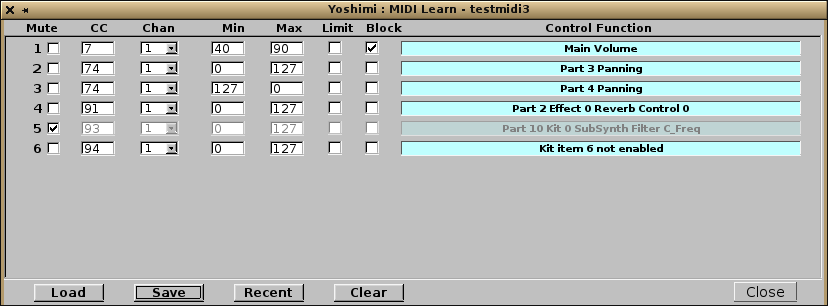
\includegraphics[scale=0.75]{1.5.8/MidiLearn.png}
   \caption{MIDI Learn Dialog}
   \label{fig:midi_learn_dialog}
\end{figure}

   If the controller learned was an NRPN, this dialog will show a hexadecimal
   number in the CC field, and this item will not be editable. Notice that a small indented button will appear between the mute status and the NRPN value. If this it clicked on it will turn red indicating that it is now a 7 bit value. This is type of range is sent by some hardware synths and controllers.

   Adding or deleting rows in this dialog, or changing the CC or channel
   number, will cause the rows to be sorted again.
   \index{MIDI Learn!200 lines}
   The maximum number of MIDI-Learned lines per session is 200.

   The major items of this dialog are the editor settings available:

   \begin{enumber}
      \item \textbf{Mute}
      \item \textbf{CC}
      \item \textbf{Chan}
      \item \textbf{Min}
      \item \textbf{Max}
      \item \textbf{Limit}
      \item \textbf{Block}
      \item \textbf{Control Function}
      \item \textbf{Load}
      \item \textbf{Save}
      \item \textbf{Recent}
      \item \textbf{Clear}
   \end{enumber}

   Now click on the \texttt{Midi Learn} button, to see a new window displaying
   the recently-learned controller. Along with a number of settings, it shows
   text with precise details of this complete action.

   Also shown is an \texttt{activity} LED that flickers when the associated
   CC/channel is received.

   \setcounter{ItemCounter}{0}      % Reset the ItemCounter for this list.

   \itempar{Mute}{MIDI Learn!Mute}
   Mute.
   Disables the MIDI Learn control specified by the corresponding line of
   settings.  The control is still available, but will not be in effect.

   Values: \texttt{Checked, Unchecked}

   \itempar{CC}{MIDI Learn!CC}
   CC.
   Incoming CC.
   Provides the value of the controller that is learned.
   For example, a value of 7 indicates the control value that would normally
   affect the main volume of \texttt{Yoshimi}.
   Note that NRPNs are \textsl{not included}.
   Also note that CC has no default values; the values are whatever the
   incoming learned values are.

   Values: \texttt{1 to 127}

   \itempar{Chan}{MIDI Learn!Chan}
   Chan.
   Incoming channel number.
   Note that, in the \textbf{MIDI Learn} window, the channel numbers start
   from 1,  as do all the other numbers in that window except controllers, which
   start from 0, following MIDI convention.
   Also note that the channel has no default values; the values are whatever the
   incoming learned values are.

   Values: \texttt{1 to 16, and All}

   \itempar{Min/Max}{MIDI Learn!Min/Max}
   Min and Max.
   Provides the minimum and maximum incoming values for the controller value.
   Since V 1.5.2 this is shown as a percentage with a resolution of 0.5
   If \textbf{Min} is greater than \textbf{Max}, this reverses the control
   direction.
   If \textbf{Min} is equal to \textbf{Max}, it becomes a threshold setting.
   Any value lower than this threshold will be passed on as 0, and any
   value higher will be passed on as 127.
   These values will then be translated to the
   \textbf{Min} and \textbf{Max} of whatever
   controller has been linked. Thus, for a simple switch those values
   will be 0 (off) and 1 (on). For most controls it will be 0 and 127.
   For an Addsynth modulator it will be OFF and PWM.

   Bear in mind that \textbf{Min} and \textbf{Max} are percentage values, not
   0-to-127 MIDI values.  Divide the incoming MIDI value by 1.27 to get the
   percentage value.  The resolution is to the nearest 0.5.
   To summarize:

   \begin{enumerate}
      \item In MIDI Learn, set both \textbf{Min} and \textbf{Max} to the same
         percentage value.  Call it "M\%".
      \item Multiply \texttt{M\%} by 1.27, and increase the result up to the
         next integer value.
   \end{enumerate}

   For example, if \texttt{M\% = 90.0}, any MIDI value $\leq$ 115 will turn a
   switch off, and any value $>$ 115 will turn it on.

   Values: \texttt{0 * (min) to 100 * (max)}

   \itempar{Limit}{MIDI Learn!Limit}
   Limit/Compression switch.
   Limiter versus compression.
   The Min/Max range can either be in the style of a limiter or a compression.
   Set to \textbf{limit}, the \textbf{Min} and \textbf{Max} will be hard
   cutoffs.
   For example, if \textbf{Min} is 20 and the incoming value is 5, then the
   result is 20.

   Set to \textbf{compress}, the incoming value will be converted to fit
   the range. For example, if \textbf{Min} is 32, \textbf{Max} is 95, then
   an incoming value of 0 will be 32, an incoming value of 2
   will be 33, etc.

   Values: \texttt{Checked (Limit), Unchecked (Compress)}

   \itempar{Block}{MIDI Learn!Block}
   Block.
   Specifies blocking of all later actions on the same CC/channel pair
   (including system ones).
   If a loaded set refers to \textsl{Yoshimi} controls that are disabled, or
   don't exist, such controls will be ignored.
   The \textsl{block} feature will be active unless the line is muted.

   Values: \texttt{Checked, Unchecked}

   Also, for devices that send high resolution controllers as NRPNs, the lines default to having \textbf{Block} set. This is so that the NRPN is not passed
   on to \textsl{Yoshimi}, which would result in "go away" messages or obscure
   actions. However, like ordinary CCs, they will stack and one can set several
   lines with the same NRPN performing multiple actions, and then unblock all
   but the last one.

   The way this fits in with the rest is that the incoming data values are
   combined as a 14 bit number, then (as a floating point number) divided by
   128 so the overall range is exactly the same as normal CCs.  However, when
   decoded for various controls *all* CCs are converted by a second (hidden)
   set of limits to get the maximum possible resolution:

   \begin{itemize}
      \item \textbf{Part}: 1 to 16
      \item \textbf{Engine fine detunes}: -8192 to 8191
      \item \textbf{Engine coarse detunes}: -64 to 63
      \item \textbf{LFO frequency}: 0.0 to 1.0 (float)
   \end{itemize}

   The actual resolution is determined by the physical control
   source. Most controls seem to be 10 bit, but if generated within an
   automation source, one will get the full 14 bits.

   \itempar{Control Function}{MIDI Learn!Control Function}
   Control function.
   Provides text describing what control is affected, or if the
   part is disabled or not.

   One can delete any existing MIDI Learn via
   \texttt{Ctrl-right-click}
   on the
   \texttt{Control Function} text for that line.
   One is then presented with a confirmation message giving the line number and
   the text as a reminder.
   Adding lines, or changing either CC or channel numbers, will
   re-order the lines.
   Deleting lines will cause a redraw, but not a re-sort.
   Changing the CC or channel will only do a re-sort when necessary, as when the
   new number is now higher or lower than the adjacent ones.

   The same CC/controller can be used to change several different internal
   \texttt{Yoshimi} controls.  For example, one can have a part's volume being
   changed while another part is having an effect level changed.
   This is done by selecting one part, and making a setting with the desired
   controller, and then selecting another part, and making a setting with the
   same controller.
   This single controller will then affect both parts at once.

   \itempar{Load}{MIDI Learn!Load}
   Load.
   Loads a set of MIDI Learn values from a file.
   The extension of the file is \texttt{.xly}.
   If a loaded set refers to \texttt{Yoshimi}
   controls that are disabled, or don't exist, those controls will be ignored.
   However the Block feature will still be active, unless the line is muted.

   \itempar{Save}{MIDI Learn!Save}
   Save.
   A complete list of MIDI Learn values
   will be saved by clicking on the Save button; one then sees
   the usual file-chooser window.
   The file is saved where desired, with the extension \texttt{.xly},

   \itempar{Recent}{MIDI Learn!Recent}
   Recent.
   This button is used for loading a set of
   MIDI Learn values from the recent history.

   \itempar{Clear}{MIDI Learn!Clear}
   Clear.
   This button clears the entire learned list from the
   \textbf{MIDI Learn} dialog.

% To come:
% Paging of the display to avoid scrolling through a massive list.

\subsection{MIDI Learn / Tutorial}
\label{subsec:midi_learn_tutorial}

   \textsl{This mini-tutorial is courtesy of Will.}

   Say one has a foot pedal that outputs CC values on the standard volume, CC 7.
   Now this is per channel, so only instruments on the first channel will pick
   it up.  This presents a problem if one has automation/backing tracks on
   other channels and one wants to keep everything together. So here is what to
   do:

   While holding down \texttt{Ctrl}, right-click on the
   \textbf{Volume} knob at the top of the
   main window. A window will open with the message "Learning Main Volume".
   If one now operates the foot pedal, the window will disappear and one will
   see that the main volume control is now responding to the foot pedal.

   \textsl{However}, this means one is changing both the main volume
   \textsl{and} the part 1 volume at the same time.  So now open the
   \textbf{MIDI learn} window via the \textbf{Yoshimi} button. One will
   see that it now has a line detailing the incoming CC and channel, along with
   other controls and the control function named \textbf{Main Volume}.  Click
   on the \textbf{Block} check box, and one will see that the part 1 volume
   control no longer responds.

   Now the foot pedal will control \textsl{only} the master volume, not the
   individual part volumes. This setup will survive loading new patch sets, and
   also a main reset (while still running).

   It's quite likely that the foot pedal will go from 0 to 127, when one actually
   wants a much smaller control range.  In that case, one can change the
   \textbf{Min} and \textbf{Max}
   values to (for example) 40 and 90.
   In this way, the entire range of the pedal control will be reduced linearly to
   40-90.

   If one sets the \textbf{Limit} checkbox, then these values will instead be
   cutoff points so anything from the pedal between 0 and 40 will be 40, and
   anything between 90 and 127 will be 90

   To temporarily disable this controller line, use the \textbf{Mute} checkbox.
   The entire line will be greyed, and as the \textbf{Block} is no longer
   active normal part volume control will be restored.

   A point that is not obvious is that although incoming CCs are per-channel,
   the actions are per-\textsl{part}, so if one sets controller 94 for part 1
   volume and then set it again for part 2 volume, one gets \textsl{two} lines,
   each controlling a different part but \textsl{acting together}.  Change the
   \textbf{Min} and \textbf{Max} of one of them to 127 and 0 respectively and
   one will increase in volume while the other reduces.

   Volume, pan, and most of the effects are \textsl{immediate}, while most of
   the other controls start on the \textsl{next note}.  Eventually it would be
   nice to get filters etc. to be immediate, but that's for another release!

%-------------------------------------------------------------------------------
% vim: ts=3 sw=3 et ft=tex
%-------------------------------------------------------------------------------
